\documentclass[tikz,border=2mm]{standalone}
\begin{document}
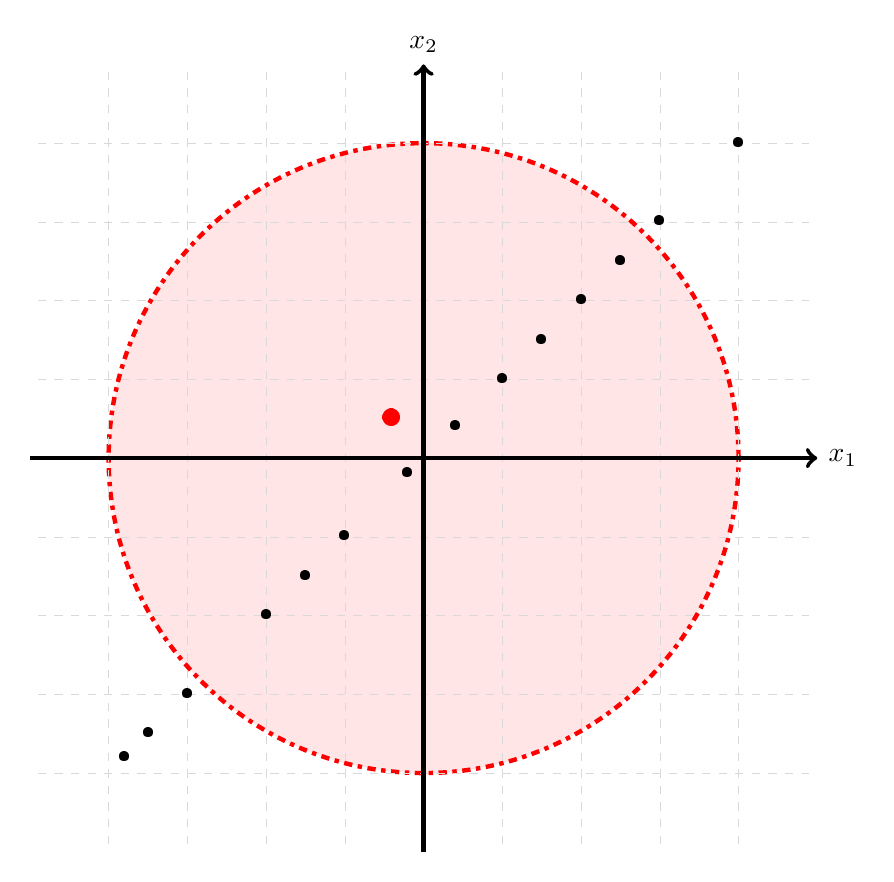
\begin{tikzpicture}
\draw[ultra thick, color=red, fill=red!10, dashdotted] (0,0) circle (4cm);
\draw[help lines, color=gray!30, dashed] (-4.9,-4.9) grid (4.9,4.9);
\draw[->,ultra thick] (-5,0)--(5,0) node[right]{$x_1$};
\draw[->,ultra thick] (0,-5)--(0,5) node[above]{$x_2$};

\node at (-3.8,-3.8){\textbullet}; 
\node at (-3.5,-3.5){\textbullet}; 
\node at (-3.0,-3.0){\textbullet}; 
\node at (-2.0,-2.0){\textbullet}; 
\node at (-1.5,-1.5){\textbullet}; 
\node at (-1.0,-1.0){\textbullet}; 
\node at (-0.2,-0.2){\textbullet}; 
\node at (0.4,0.4){\textbullet}; 
\node at (1.0,1.0){\textbullet}; 
\node at (1.5,1.5){\textbullet}; 
\node at (2.0,2.0){\textbullet}; 
\node at (2.5,2.5){\textbullet}; 
\node at (3.0,3.0){\textbullet}; 
\node at (4.0,4.0){\textbullet}; 

\node[color=red] at (-0.4,0.5){\LARGE\textbullet}; 

\end{tikzpicture}
\end{document}
